\documentclass{article}
\usepackage{geometry}

\geometry{a4paper,left=2cm,right=2cm,top=1cm,bottom=1.5cm}
\usepackage{xeCJK, fontspec, xunicode, xltxtra}  
\usepackage[colorlinks,
            linkcolor=blue,
            anchorcolor=blue,
            citecolor=blue
            ]{hyperref}
%\setCJKmainfont{Hiragino Sans GB}  
\setmainfont{Times New Roman}  
\setCJKmainfont{Songti SC}

\usepackage{graphicx} 
\usepackage{amsmath}
\usepackage{amssymb}

\usepackage{listings}
\usepackage{xcolor}
\lstset{
    numbers=left, 
    numberstyle= \tiny, 
    keywordstyle= \color{ blue!70},
    commentstyle= \color{red!50!green!50!blue!50}, 
    frame=shadowbox, % 阴影效果
    rulesepcolor= \color{ red!20!green!20!blue!20} ,
    escapeinside=``, % 英文分号中可写入中文
    xleftmargin=2em,xrightmargin=2em, aboveskip=1em,
    framexleftmargin=2em
} 


\title{2016060104002\_2017060103023\_2}
\author{Haodong Liao \& Fan Gao}

\begin{document}
\maketitle{}

% \quad Having changed the class of Coursera course : Interactive Computer Graphics by Takeo Igarashi of The University of Tokyo to June 25, I have to wait until then. And due to the final exam of 3D Graphic Programming, I didn't get the time to study the Coursera course : Introduction to C\# Programming and Unity by  Dr. Tim "Dr. T" Chamillard of The University of Colorado either.

% \section{The tasks I have done last week}
% \begin{itemize}%项目符号开始

% %\item Having changed the class of Coursera course : Interactive Computer Graphics by Takeo Igarashi of The University of Tokyo to June 25, I have to wait until then. And due to the final exam of 3D Graphic Programming, I didn't get the time to study the Coursera course : Introduction to C\# Programming and Unity by  Dr. Tim "Dr. T" Chamillard of The University of Colorado either.

% %\item I've submited my curriculum design.

% %\item I'm studying a Coursera course:Introduction to C\# Programming and Unity by  Dr. Tim "Dr. T" Chamillard of The University of Colorado,and finished the study of Week 1.

% %\item I've taken the final exam of the mathematical modeling course.

% %\item I'm participated in the summary defense of the student union of the youth league committee of the school of computer science and engineering.

% \item I have been reviewing the final exam of 3D Graphic Programming.


% \end{itemize}

% \section{My plan for next week}

% \noindent
% \qquad I plan to do things as follows:

% \begin{itemize}

% \item Finish the Week2 course of Introduction to C\# Programming and Unity by  Dr. Tim "Dr. T" Chamillard of The University of Colorado

% \item Review the final exam of Database.
% \item Review the final exam of Computer Network.
% \item Review the Rebuilt test of Calculus 1 \& 2.

% \end{itemize}

\section{Preface}

This was a \LaTeX report written by Haodong Liao and Fan Gao, students of UESTC who participated in the summer school of UCPH. More codes of this summer school were at this \href{https://github.com/Medill-East/ComputerScience/tree/master/Professional%20Core%20Courses/Functional%20Programming/SummerSchool/Advanced%20Functional%20Programming/AdvancedFunctionalProgramming/AdvancedFunctionalProgramming}{repository}.

\section{Introduction}

Little Claus and Big Claus (Danish: Lille Claus og store Claus) is a tale about a poor farmer, who outsmarts a rich farmer\footnote[1]{http://andersen.sdu.dk/vaerk/hersholt/LittleClausAndBigClaus\_e.html}. After analyzing and generating target text according to the story's statistics last week, it was time to move on.

In this assignment, we designed a spell checker which was based on the text by H.C. Andersen. In detail, we used pattern-matching, currying, higher-order function and other powerful tools to complete our functions to meet the requirements, which gave us a sense of accomplishment. 

% All in all, the results I achieved were as following:

% \begin{itemize}
% \item met the requirement of replacing the library calls in \emph{myFold} and \emph{myFilter} with my own recursive implementations of these functions,
% \item used \emph{match..with} to achieved pattern-matching,
% % \item made the program work on my own and improved \emph{myFold} function to be more generic with the help of Prof.Sporring.
% \end{itemize}

% The remaining structure of the article is as follows. Section 3 states the problem in detail. Section 4 analysis and designs the problem. Section 5 describes the essential parts of my implementation. The program is evaluated in Section 6 and discussed in Section 7.

% \section{Problem statement}

% This assignment required us to replace the library function with recursive implementations for \emph{myFold} and \emph{myFilter} based on the file \emph{recursiveMapFoldFilter.fsx}, which is a fully functioning program must be compiled and executed from the console. 

% This program takes 2 arguments: a string and a positive integer \emph{n}. The string can be either \emph{map}, \emph{fold}, or \emph{filter}. The output is a random list of length \emph{n} consisting of positive integers less than 10 and a processed list. For \emph{fold}, the random elements have been multiplied by 2 and their order has been reversed, and for \emph{filter}, only those elements larger than 4 have been included.

\section{Analysis and Design}

% \subsection{Text Processing of character}
\subsection{Understand the data structure Trie}
% \lstset{language=Csh}
\begin{lstlisting}
type Trie<'T when 'T : comparison> = {
    IsTerminal: bool;               
    Children: Map<'T, Trie<'T>>;}
\end{lstlisting}

As explained by Prof.Düdder, we would build a "forest" at the end, which meant when we got a "root", there was a whole "word forest" behind it. If the subtree made up a word, \emph{IsTerminal} was true.

\subsection{Lookup Function}\label{sec:lookup}

% \lstset{language=Csh}
\begin{lstlisting}
lookup (prefix: string) (trie: Trie<char>) : Trie<char> Option
\end{lstlisting}

It was a preparation for completing the \emph{autoComplete} function. In this function worked well, if the \emph{prefix} was "ab", then it should return things like "abstract", "absolute" and so on. Which meant there were two branches to be handled when we match the pattern of \emph{prefix}. If it was empty, then \emph{None} should be the output option, else the output should be the option of a trie. To meet the requirement, we could use the \emph{find} function provided in the material. The key part of the pseudocode was shown as following:

\begin{lstlisting}
let lookup (prefix: string) (trie: Trie<char>) : Trie<char> Option = 
    match prefix with
    | empty -> None
    | not empty -> use "find" function to return the option of a trie
\end{lstlisting}

\subsection{AutoComplete Function}\label{sec:autocomplete}
% \lstset{language=Csh}
\begin{lstlisting}
autoComplete (prefex: string) (trie: Trie<char>) : string seq
\end{lstlisting}

The goal of this sub-assignment was to return an option of the (sub)trie found by the \emph{lookup} function, if the word began with the \emph{prefix} exists, after which \emph{autoComplete} function should return a sequence of strings of words which \emph{prefix} in the trie.

Same as \emph{lookup}, there were two branches needed to be handled, if the \emph{prefix} argument was empty, then we returned an empty sequence, else we \emph{lookup} the target option of a trie and returned it. The key part of the pseudocode is shown as following:

\begin{lstlisting}
let autoComplete (prefix: string) (trie: Trie<char>) : string seq = 
    match prefix with
    | empty -> returns an empty sequence
    | str -> 
        match (result of "lookup" function) with
            | Not find -> returns an empty sequence
            | Some x -> returns the sequence
\end{lstlisting}

\subsection{SpellCheck Function}\label{sec:spellcheck}
% \lstset{language=Csh}
\begin{lstlisting}
spellCheck (word: string) (trie: Trie<char>) : bool
\end{lstlisting}

We needed to check if a word was correct by checking containment in the given trie. Thanks to the \emph{contains} function given in the material, we could meet the requirement simply by taking the \emph{word} argument as the parameter of \emph{contains} function. The key part of the pseudocode was shown as following:

\begin{lstlisting}
let spellCheck (word: string) (trie: Trie<char>) : bool = 
    contains word trie
\end{lstlisting}

\subsection{Generate Random Word}\label{sec:randword}
% \lstset{language=Csh}
\begin{lstlisting}
randWord (trie: Trie<char>): char list
\end{lstlisting}

This sub-assignment required to pick a random word from the given trie, and this was the preparation part of \emph{genText} function. The key to this sub-task was to get the "word library" first and pick a word randomly from it. The key part of the pseudocode was shown as following:

\begin{lstlisting}
let randWord (trie: Trie<char>) : char list = 
    Get the "word library"
    Generate a random number whose scope covers the entire vocabulary
    Pick a word according to the random number (the position of the word)
\end{lstlisting}

\subsection{Generate a text}\label{sec:gentext}
% \lstset{language=Csh}
\begin{lstlisting}
genText (len:int) (trie: Trie<char>) : string
\end{lstlisting}

In this sub-assignment, we needed to generate a text based on a length \emph{len} and \emph{trie}, the result was a string consisting of \emph{len} words drawn out of the trie.

The tricky part of this sub-task was how to handle the linked part between words and the last word. The solution was that there should be a "space" between two words and we should deal with the last word separately. So there were three branches to be handled, i.e., \emph{len} was bigger than one, \emph{len} was equal to one. Other situations should be taken as an error. The key part of the pseudocode was shown as following:

\begin{lstlisting}
let rec genText (len: int) (trie: Trie<char>) : string =
    match len with
    | x when x > 1 -> Generate and concatenate the words
    | 1 -> Generate the last word
    | _ -> Error situations
\end{lstlisting}

\section{Program description}
\subsection{Lookup Function}

Our implementation of \textbf{lookup} function was as follows:

\begin{lstlisting}
let lookup (prefix: string) (trie: Trie<char>) : Trie<char> Option = 
    match prefix with
    | "" -> None
    | str -> find (stringToCharlist str) trie    
\end{lstlisting}

As described in \ref{sec:lookup}, the key to this function was to take advantage of the \emph{find} function. To do that, we needed to create our own \emph{stringToCharlist} function so to make the \emph{prefix} argument meet the requiremnt. And the implementation of \textbf{stringToCharlist} function was as follows: 

\begin{lstlisting}
let rec stringToCharlist (input: string) : char list = 
    match input with
    | "" -> []
    | str -> str.[0]::(stringToCharlist str.[1..])     
\end{lstlisting}

\subsection{AutoComplete Function}

Implementation of \textbf{autoComplete} function was as follows:

% \lstset{language=Csh}
\begin{lstlisting}
let autoComplete (prefix: string) (trie: Trie<char>) : string seq = 
    match prefix with
    | "" -> Seq.empty
    | str -> 
        try
            match (lookup str trie) with
            | Option.None -> Seq.empty
            | Some x -> Seq.map (fun x-> x.ToString()) (trieToSeq trie)
        with
            | ex -> eprintf "An exception occurred with message 
                    Seq.empty
\end{lstlisting}

As described in \ref{sec:autocomplete}, to complete the string correctly, we needed to match the pattern of \emph{prefix}, for \emph{prefix} with content, we use \emph{try..with} method to make sure everything go well. In the \emph{try} part, we match the result of \emph{lookup} function with two branches, and we used \emph{Seq.map} to change the \emph{Seq<char list>} to \emph{Seq<string>}.

\subsection{SpellCheck Function}

Implementation of \textbf{spellCheck} function was as follows:

% \lstset{language=Csh}
\begin{lstlisting}
let spellCheck (word: string) (trie: Trie<char>) : bool = 
    contains (stringToCharlist word) trie
\end{lstlisting}

As described in \ref{sec:spellcheck}, it was not hard for us to use the given \emph{contains} function to complete this sub-task. And all we needed to do was to convert the \emph{word} argument to \emph{char list} so everything goes well.

\subsection{Generate Target Text}

Implementations of \textbf{randWord} and \textbf{genText} function were as follows:

% \lstset{language=Csh}
\begin{lstlisting}
let randWord (trie: Trie<char>) : char list = 
    let wordList = Seq.toList (trieToSeq trie)  //char list list
    wordList.[Random().Next(1,wordList.Length)] // char list

let rec genText (len: int) (trie: Trie<char>) : string =
    match len with
    | x when x > 1 -> (charlistToString (randWord trie)) 
                      + " " + (genText (x-1) trie)
    | 1 -> (charlistToString (randWord trie))
    | _ -> "Error"
\end{lstlisting}

As described in \ref{sec:randword} and \ref{sec:gentext}, to generate a target text, the first step was to pick a word randomly from the given trie. To achieve this, we needed to get the "word library" (achieved at the first line of \emph{randWord} function) as we discussed so that we could pick the word randomly from the library (achieved at the second line of \emph{randWord} function).

The tricky part of the \emph{genText} function was that we confused about the concatenation method of \emph{string}, we used \emph{::} to joint the string and things did not work well. Then we used \emph{+} to concatenate the string and it worked this time.

Another thing we needed to do was convert the \emph{char list} to \emph{string} so that we returned the text correctly. The Implementation of \textbf{charlistToString} was as follows:

% \lstset{language=Csh}
\begin{lstlisting}
let rec charlistToString (input: char list): string = 
    match input with
    | [] -> ""
    | fst::rest -> string(fst) + charlistToString(rest)
\end{lstlisting}

\section{Evaluation}

The testing environment was macOS Mojave 10.14.5 system with iTerm and Microsoft (R) F\# Compiler version 4.1.

\subsection{Test of AutoComplete}

Except for the given positive test of \emph{"st"; "ca"; "cu"}, negative test of \emph{"gts"; "kns"; "iqw"}, we extended the \emph{"wh"; "ab"; "cl"} into the positive test, and the \emph{"ijk"; "tzw"} into the negative test, and the result of this function was shown as follows:

\begin{figure}[htbp]
      \centering
      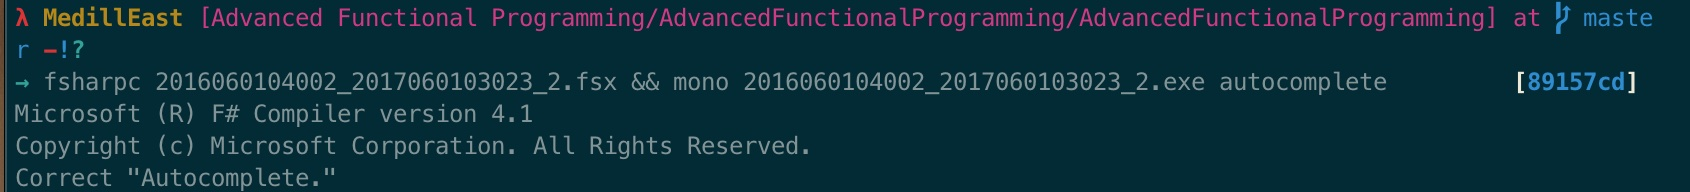
\includegraphics[width=\linewidth]{autocomplete}
      \caption{Testing of autoComplete function}
      \label{fig:autocomplete}
\end{figure}

\subsection{Test of SpellCheck}

Except for the given positive test of \emph{"standing"; "can"; "about"}, negative test of \emph{"gts"; "cfm"; "iqw"}, we extended the \emph{"one"; "four"} into the positive test, and the \emph{"txq"; "ihu"; "svv"} into the negative test, and the result of this function was shown as follows:

\begin{figure}[htbp]
      \centering
      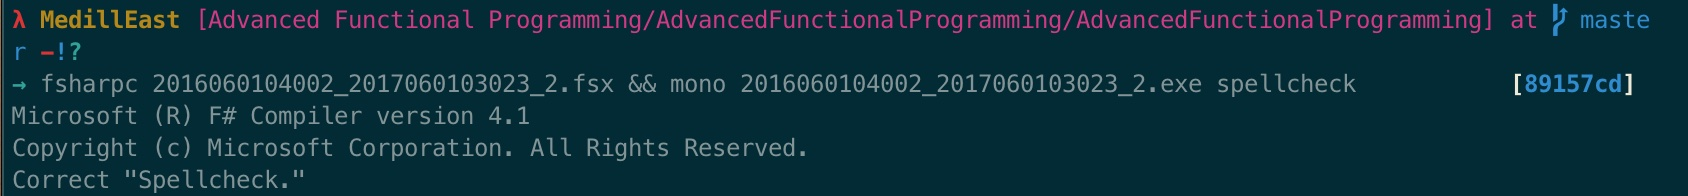
\includegraphics[width=\linewidth]{spellcheck}
      \caption{Testing of spellCheck function}
      \label{fig:spellcheck}
\end{figure}

\subsection{Test of GenerateText}

We test the function as required, and the result of this function was shown as follows:

\begin{figure}[htbp]
      \centering
      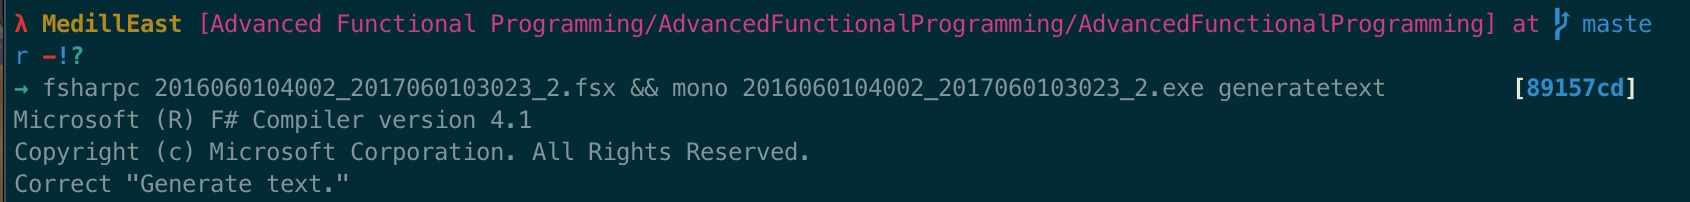
\includegraphics[width=\linewidth]{generatetext}
      \caption{Testing of genText function}
      \label{fig:generatetext}
\end{figure}

% \begin{figure}[htbp]
%       \centering
%       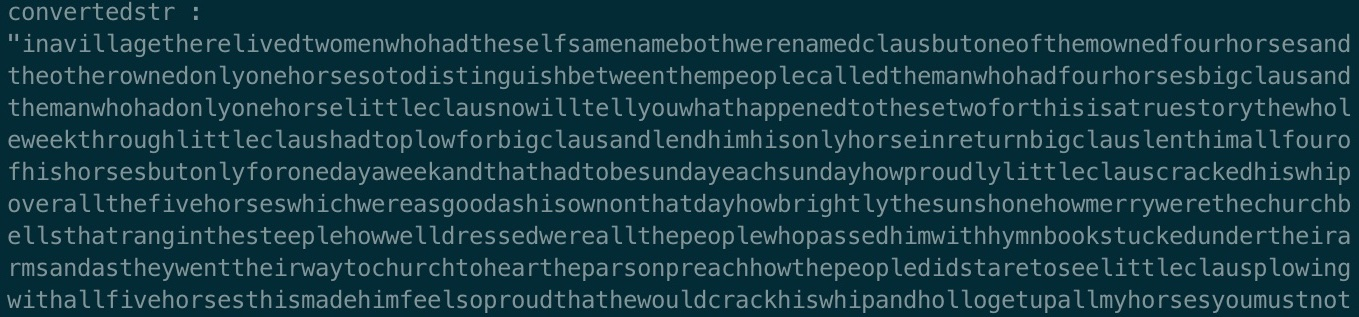
\includegraphics[width=\linewidth]{convert}
%       \caption{Testing of convertText function}
%       \label{fig:convert}
% \end{figure}

% \begin{figure}[htbp]
%       \centering
%       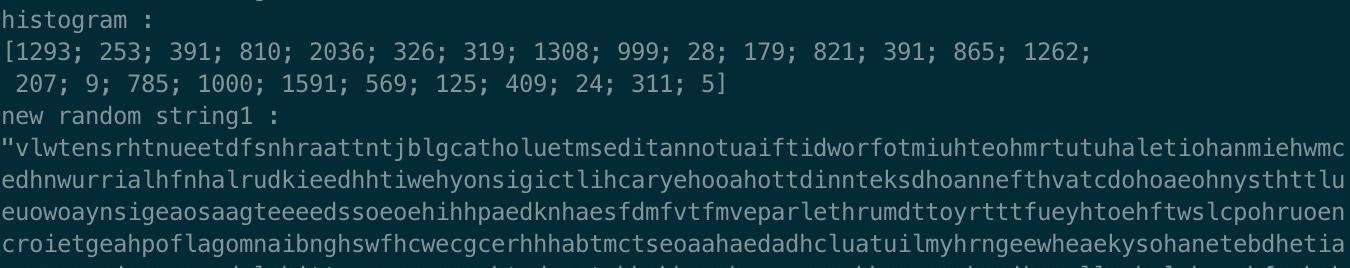
\includegraphics[width=\linewidth]{histogramandnewstring1}
%       \caption{Testing of histogram and randomString function}
%       \label{fig:histogramandnewstring1}
% \end{figure}

% \begin{figure}[htbp]
%       \centering
%       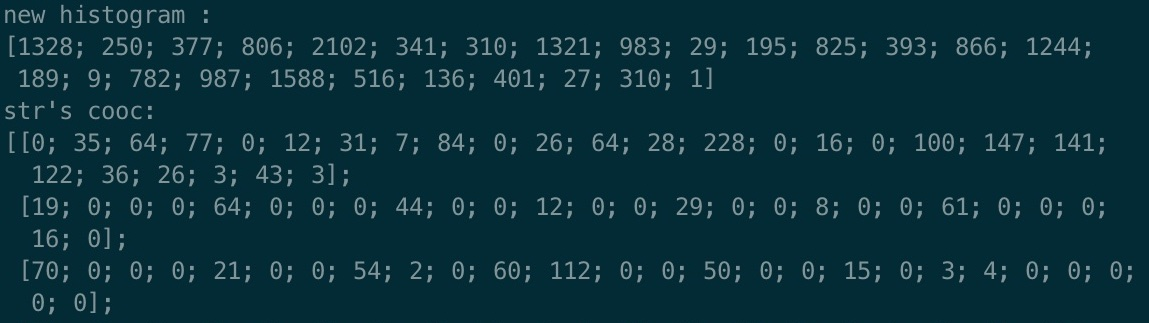
\includegraphics[width=\linewidth]{newhistogram1andoldcooc}
%       \caption{Histogram and Cooc of Generate String of randomString function}
%       \label{fig:newhistogram1andoldcooc}
% \end{figure}

\section{Discussion \& Conclusion}

As shown above, all of our function worked well as expected.

In this assignment, we designed a spell checker which was based on the text by H.C. Andersen. Thanks to the given powerful function, all we had to do was to figure out the conversion of different types, which reminds us that it is very important to use tools properly to work efficiently. How time flies, yesterday I had to worry about the program, and at this moment we are about to part. It is our pleasure to have Prof.Düdder as our teacher and Sarah as our teaching assistant, and we believe that we had a good time. Many thanks!


%\renewcommand\refname{Reference\\
%\small those are reference form Week 6, I'll list Week5's reference next time}

% \bibliographystyle{unsrt}
% \bibliography{reference}

%\begin{thebibliography}{99}
%\bibitem{1} \href{http://research.nii.ac.jp/~takayama/metallophone/metallophone-cga2011.pdf}{Responsive FEM for Aiding Interactive Geometric Modeling} \\
%Umetani N, Takayama K. Responsive FEM for Aiding Interactive Geometric Modeling[J]. 2010.

%\bibitem{2} \href{http://www-ui.is.s.u-tokyo.ac.jp/~takeo/papers/umetani_nime2010_metallophone.pdf}{Designing Custom-made Metallophone with Concurrent Eigenanalysis}\\
%Umetani N, Mitani J, Igarashi T. Designing Custom-made Metallophone with Concurrent Eigenanalysis[J]. Data, 2010. 

%\bibitem{3} \href{http://www.jst.go.jp/erato/igarashi/publications/001/SensitiveCouture.pdf}{Sensitive Couture for Interactive Garment Modeling and Editing}\\
%Umetani N, Kaufman D M, Igarashi T, et al. Sensitive couture for interactive garment modeling and editing[C]// ACM, 2011:1-12.

%\bibitem{4} \href{http://www.jst.go.jp/erato/igarashi/en/projects/GuidedExploration/2012_siggraph_GuidedExploration.pdf}{Guided Exploration of Physically Valid Shape for Furniture Design}\\
%Umentani N, Igarashi T, Mitra N J. Guided exploration of physically valid shapes for furniture design[J]. Communications of the ACM, 2015, 58(9):116-124.

%\bibitem{5} \href{http://www.nobuyuki-umetani.com/publication/2014_sigg_pteromys/2014_siggraph_GliderDesign.pdf}{Pteromys: Interactive Design and Optimization of Free-formed Free-flight Model Airplanes}\\
%Umetani N, Koyama Y, Schmidt R, et al. Pteromys:interactive design and optimization of free-formed free-flight model airplanes[J]. Acm Transactions on Graphics, 2014, 33(4):1-10. 

%\bibitem{6} Mori Y, Igarashi T. Plushie: an interactive design system for plush toys[C]//ACM Transactions on Graphics (TOG). ACM, 2007, 26(3): 45.

%\bibitem{7} Igarashi Y, Igarashi T, Mitani J. Beady: interactive beadwork design and construction[J]. ACM Transactions on Graphics (TOG), 2012, 31(4): 49.
 
%\bibitem{8} Saul G, Lau M, Mitani J, et al. SketchChair: an all-in-one chair design system for end users[C]//Proceedings of the fifth international conference on Tangible, embedded, and embodied interaction. ACM, 2011: 73-80.
 
%\bibitem{9} Saakes D, Cambazard T, Mitani J, et al. PacCAM: material capture and interactive 2D packing for efficient material usage on CNC cutting machines[C]//Proceedings of the 26th annual ACM symposium on User interface software and technology. ACM, 2013: 441-446.

% \bibitem{10} A. Rovira, D. Swapp, B. Spanlang, and M. Slater. The use of virtual reality in the study of people’s responses to violent incidents. Frontiers in Behavioral Neuroscience, 3(59), 2009. doi: 10.3389/neuro.08.059.2009
 %\bibitem{11} J.Russell.Agency:itsroleinmentaldevelopment.EssaysinEnvironmen- tal Psychology. Psychology Press, East Sussex, UK, 1996.
 %\bibitem{12} R.Skarbez.Apreliminaryinvestigationofplaceillusionandplausibility illusion. In IEEE Virtual Reality (VR) Doctoral Consortium, 2015.
 %\bibitem{13} M.Slater.Placeillusionandplausibilitycanleadtorealisticbehaviorin immersive virtual environments. Philosophical transactions of the Royal Society of London. Series B, Biological sciences, 364:3549–3557, 2009.
 %\bibitem{14} M. Slater, P. Khanna, J. Mortensen, and I. Yu. Visual realism enhances realistic response in an immersive virtual environment. IEEE Computer Graphics and Applications, 29:76–84, 2009. doi: 10.1109/MCG.2009.55
 %\bibitem{15} M. Slater, B. Spanlang, and D. Corominas. Simulating virtual environ- ments within virtual environments as the basis for a psychophysics of presence. ACM Trans. Graph., 29:92:1–92:9, July 2010. doi: 10.1145/ 1778765.1778829
 
%\end{thebibliography}



\end{document}